\documentclass[tikz, border=15pt]{standalone}
\usepackage[utf8]{inputenc}
\usepackage[T5]{fontenc}
\usepackage{lmodern}
\usepackage{xcolor}
\usepackage{graphicx}
\usetikzlibrary{positioning, calc, arrows}

\begin{document}
\begin{tikzpicture}[
  >=stealth,
  font=\sffamily,
  % Khung cột nét đứt to rõ trên nền trắng tinh
  tierColumn/.style={
    draw=black,
    dashed,
    line width=1.2pt,
    fill=white,
    rounded corners=6pt,
    inner sep=10pt,
    text width=5.2cm,
    minimum height=9.6cm,
    align=center
  },
  % Khung nhỏ bên trong
  innerBox/.style={
    draw=black!75,
    dashed,
    line width=0.9pt,
    fill=white,
    rounded corners=4pt,
    inner sep=5pt,
    align=center
  },
  % Mũi tên to rõ nét
  arrowThick/.style={
    ->,
    line width=1.8pt,
    draw=black
  },
  biArrowThick/.style={
    <->,
    line width=1.8pt,
    draw=black
  },
  % Nhãn trên mũi tên to rõ, dễ đọc
  tagText/.style={
    font=\small\bfseries,
    fill=white,
    inner sep=3.5pt,
    rounded corners=2pt,
    draw=gray!30,
    line width=0.5pt,
    text=black
  }
]

% ==================== 4 CỘT KIẾN TRÚC NẰM NGANG (LANDSCAPE) ====================

% CỘT 1: TẦNG ĐEO
\node[tierColumn] (col1) at (-9.6, 0) {
  {\bfseries\large TẦNG 1: TẦNG ĐEO}\\[2pt]
  {\footnotesize (Wearable Tier)}\\[8pt]
  
  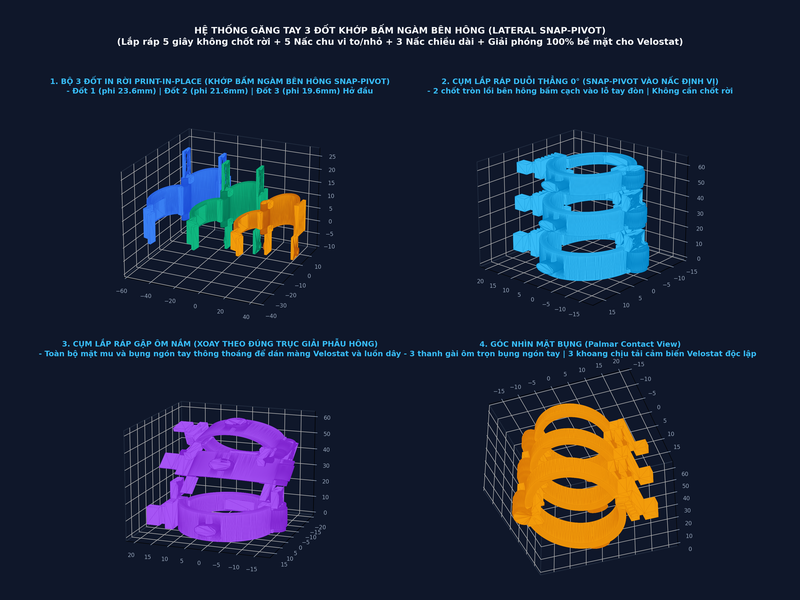
\includegraphics[width=4.8cm, height=3.0cm, keepaspectratio]{assets/splint_3d.png}\\[4pt]
  {\bfseries\small Khung nẹp 3 ngón in 3D}\\[2pt]
  {\footnotesize Ngàm xoay 2 bản lề đóng 1 tay}\\[8pt]
  
  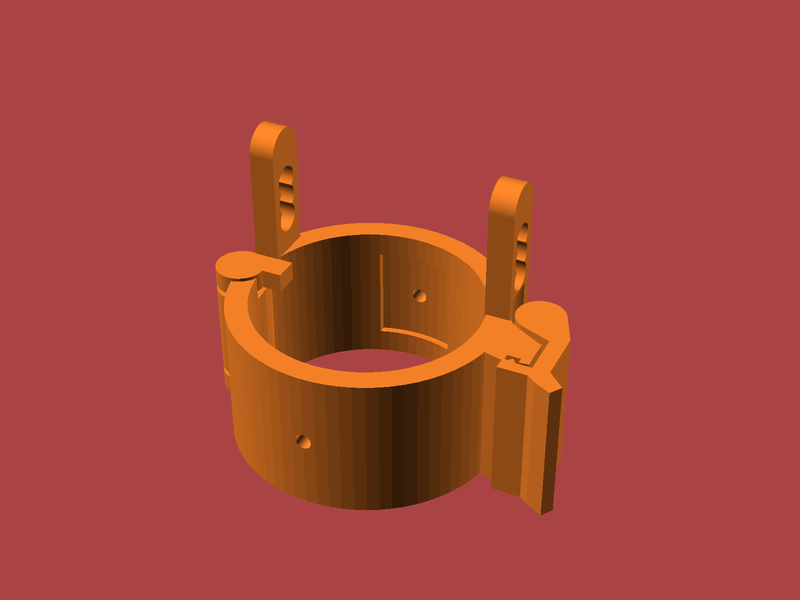
\includegraphics[width=4.8cm, height=2.2cm, keepaspectratio]{assets/mech9.png}\\[4pt]
  {\bfseries\small Cảm biến tiếp xúc \& góc}\\[2pt]
  {\footnotesize 16 Ô Velostat vi sai + 3 Flex}
};

% CỘT 2: TẦNG THU THẬP & DSP
\node[tierColumn, right=38pt of col1] (col2) {
  {\bfseries\large TẦNG 2: THU THẬP \& DSP}\\[2pt]
  {\footnotesize (Sensing \& DSP Tier)}\\[8pt]
  
  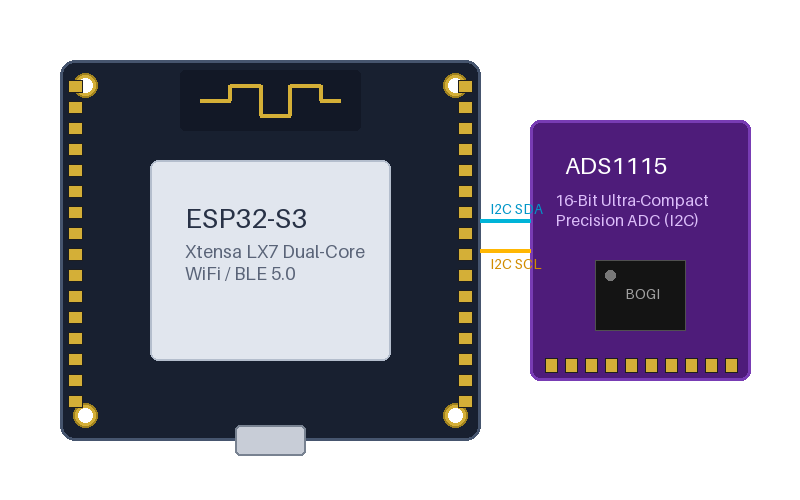
\includegraphics[width=4.8cm, height=2.8cm, keepaspectratio]{assets/controller_ads_board.png}\\[4pt]
  {\bfseries\small ESP32-S3 + ADS1115 (16-bit)}\\[2pt]
  {\footnotesize 2 MUX CD74HC4067 (21 kênh $\ge$15Hz)}\\[8pt]
  
  \begin{tikzpicture}
    \node[innerBox, text width=4.5cm] {
      {\bfseries\small Xử lý tín hiệu số (DSP)}\\[2pt]
      {\scriptsize $\bullet$ Bám nền động khử trôi tĩnh}\\[2pt]
      {\scriptsize $\bullet$ Ngưỡng thích nghi 180 mV vi sai}\\[2pt]
      {\scriptsize $\bullet$ Tính chỉ số EI -- GAP -- RAL}
    };
  \end{tikzpicture}
};

% CỘT 3: TẦNG TRỢ LỰC CƠ HỌC
\node[tierColumn, right=38pt of col2] (col3) {
  {\bfseries\large TẦNG 3: TRỢ LỰC}\\[2pt]
  {\footnotesize (Actuation Tier)}\\[8pt]
  
  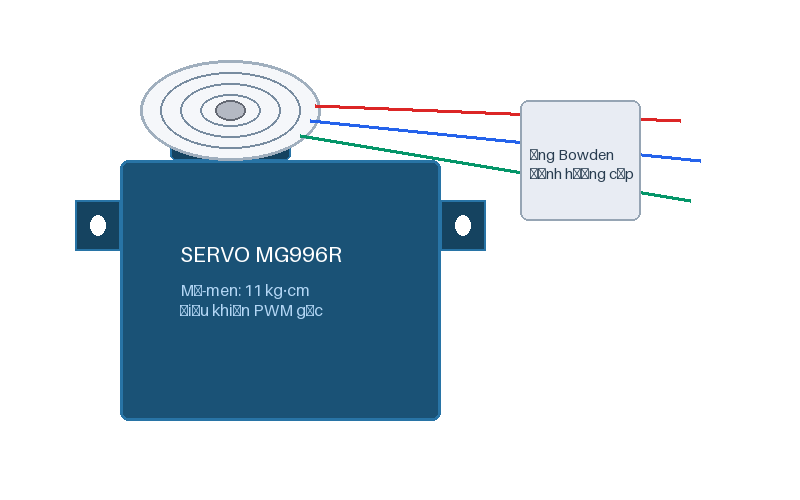
\includegraphics[width=4.8cm, height=3.0cm, keepaspectratio]{assets/servo_spool_assembly.png}\\[4pt]
  {\bfseries\small 3 Servo MG996R \& Tang cáp}\\[2pt]
  {\footnotesize Kéo gập chủ động độc lập 3 ngón}\\[8pt]
  
  \begin{tikzpicture}
    \node[innerBox, text width=4.5cm] {
      {\bfseries\small Cơ cấu truyền động Bowden}\\[2pt]
      {\scriptsize $\bullet$ Cáp Dyneema chịu lực kéo}\\[2pt]
      {\scriptsize $\bullet$ Servo chủ động nhả cáp duỗi}\\[2pt]
      {\scriptsize $\bullet$ Nẹp đàn hồi hồi vị mu tay}
    };
  \end{tikzpicture}
};

% CỘT 4: TẦNG THỊ GIÁC & TÁC VỤ
\node[tierColumn, right=38pt of col3] (col4) {
  {\bfseries\large TẦNG 4: THỊ GIÁC 3D}\\[2pt]
  {\footnotesize (Vision Pre-Actuation)}\\[8pt]
  
  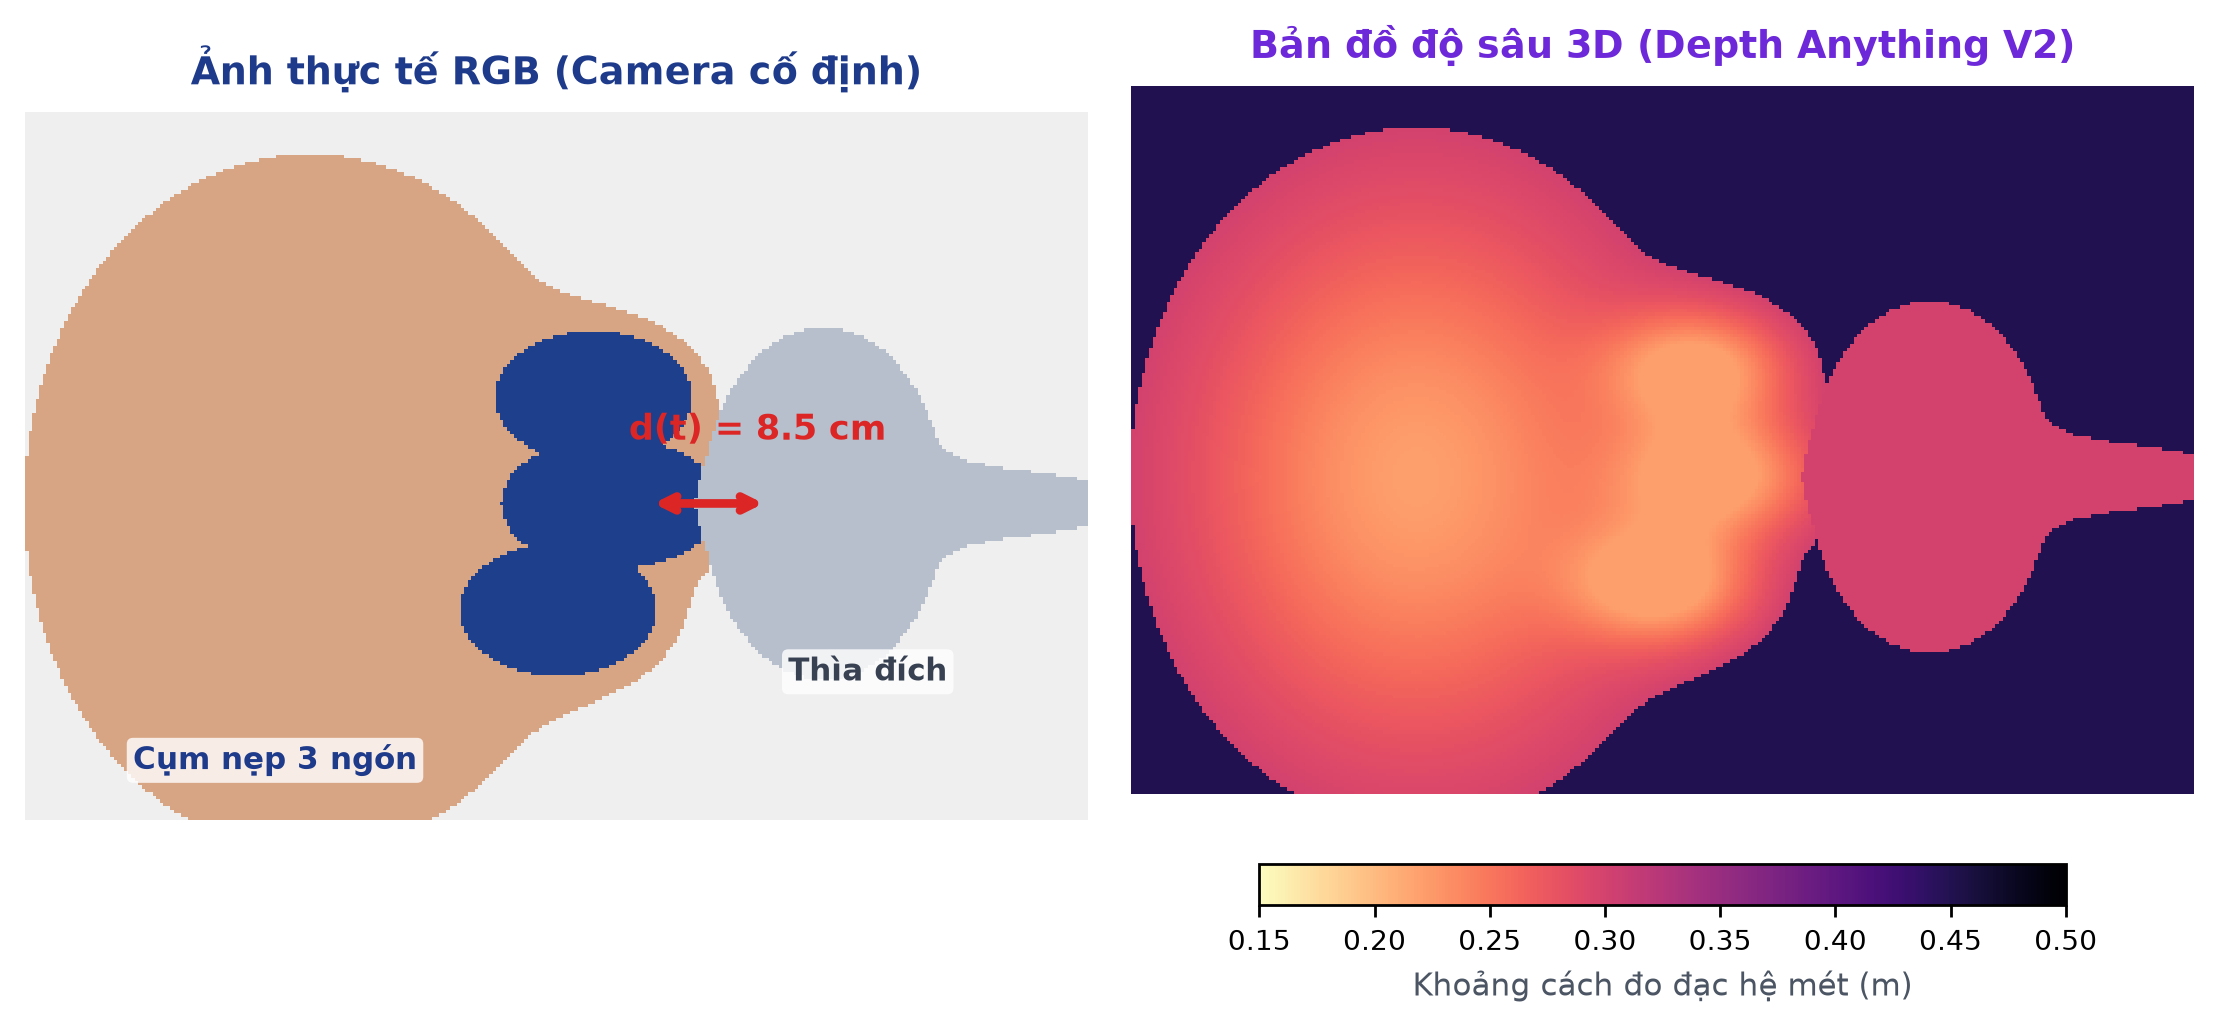
\includegraphics[width=4.8cm, height=2.8cm, keepaspectratio]{assets/depth_anything_scene.png}\\[4pt]
  {\bfseries\small Depth Anything V2 (3D)}\\[2pt]
  {\footnotesize Camera RGB + Bản đồ độ sâu hệ mét}\\[8pt]
  
  \begin{tikzpicture}
    \node[innerBox, text width=4.5cm] {
      {\bfseries\small Orange Pi 5 Pro (NPU)}\\[2pt]
      {\scriptsize $\bullet$ Ước lượng cự ly 3D tay -- thìa $d(t)$}\\[2pt]
      {\scriptsize $\bullet$ Dự báo thời gian tiếp xúc TTC}\\[2pt]
      {\scriptsize $\bullet$ Lượng hóa bài tập kẹp 3 chấu}
    };
  \end{tikzpicture}
};

% ==================== MŨI TÊN LIÊN KẾT NGANG TUYỆT ĐẸP ====================

% Tầng 1 -> Tầng 2: Tín hiệu cảm biến
\draw[arrowThick] (col1.east) -- node[tagText, above=2pt] {Tín hiệu 21 kênh} node[tagText, below=2pt] {Lực vi sai \& Góc} (col2.west);

% Tầng 2 -> Tầng 3: Lệnh servo AAN
\draw[arrowThick] (col2.east) -- node[tagText, above=2pt] {Lệnh servo AAN} node[tagText, below=2pt] {Kéo gập / Nhả duỗi} (col3.west);

% Tầng 4 <-> Tầng 2/3: Cự ly 3D và TTC
\draw[biArrowThick] (col4.west) -- node[tagText, above=2pt] {Cự ly 3D $d(t)$} node[tagText, below=2pt] {Thời gian TTC đón trước} (col3.east);

% Vòng phản hồi cơ học từ Tầng 3 quay về Tầng 1 (Vòng cung uốn dưới đáy thanh thoát)
\draw[arrowThick, dashed] (col3.south) -- ++(0, -0.9cm) coordinate (p3) -- ($(p3) - (12.8cm, 0)$) coordinate (p1) node[tagText, midway, below=3pt] {Vòng cơ học: Cáp Bowden kéo trợ lực gập ngón / Nhả duỗi mở khẩu độ} -- (col1.south);

\end{tikzpicture}
\end{document}
